\appendix
\setcounter{figure}{1}
\renewcommand{\thefigure}{A\arabic{figure}}
\setcounter{figure}{0}

\section{Details}
\label{app:details}

\paragraph{Camera mounting and aiming.}
The Arducam B0587 sits on a \$10 GoPro head strap through a printed GoPro-pattern adapter (\SI{103}{g} worn, plus \SI{37}{g} of USB cable). With the live preview open, the collector looks at a point \SI{0.5}{}--\SI{1}{m} away and tilts the mount until the centre of the frame coincides with the centre of their own view, so the camera looks where the head looks. The positioner carries the same pattern: the SO-101 follower's gripper bracket is removed and its gripper servo reused as a wrist-yaw joint, so the one camera moves between head and robot without re-mounting.

\paragraph{Calibration.}
With the ball mounted on the YAM's gripper, the flange-to-ball link is solved as a robot-world hand-eye problem (OpenCV's \texttt{calibrateRobotWorldHandEye}, \citet{shah2013robotworld}), and the tile-world-to-base link is a trimmed Kabsch fit of the head-camera tool point (tiles $\times$ ball) to forward kinematics over one 5\,065-frame session (\SI{91}{\percent} inliers). The tile refit reduces four-tile reprojection error from \SI{3.4}{px} to \SI{0.5}{px} RMS and the disagreement between single-tile solves of the same frame from \SI{10}{}--\SI{13}{mm} to \SI{4}{}--\SI{9}{mm}. Single-tile frames are chained under velocity bounds of \SI{0.6}{m/s} and \SI{120}{\degree/s}.

\paragraph{Positioner control.}
Forward kinematics gives the gripper position; a fixed-gain controller holds its initial visual bearing, and the residual model adds the head's displacement relative to the hand. The model is a ridge regression on nine pose features plus the grasp bearing, a bearing history and the distance, fitted on about 100 glove episodes of one session; on 15 held-out episodes it predicts the collector's head pose to \SI{46}{mm} / \SI{5.4}{\degree} median (\SI{81}{mm} / \SI{9.6}{\degree} p90), against \SI{87}{mm} / \SI{7.0}{\degree} for a camera held at the median head pose. Commands are low-pass filtered, rate-limited to \SI{50}{\degree/s} and bounded to a safe volume.

\section{Jaw-width accuracy by condition}
\label{app:width}
On 112 teleoperated episodes (24.6k frames) the head-camera width is compared with the encoder value. Binned by workspace quartile, by distance to the camera (\SI{0.4}{}--\SI{0.8}{m}), by the camera's elevation (\SI{40}{}--\SI{87}{\degree}) and by the angle between the line of sight and the jaw axis, every bin reads \SI{2.8}{}--\SI{4.8}{\percent} of stroke median and \SI{6.8}{}--\SI{8.5}{\percent} p90, worst when the camera looks across the jaws rather than along them. Shifting the label by one frame in either direction raises the error, so there is no lag. The residual is a systematic under-read of \SI{4}{}--\SI{6}{\percent} at full opening, a scale error of the per-session fit (alternate-frame holdout) rather than noise. The fixed camera of \citet{yamumi2026} read the same gripper at \SI{4.4}{\percent} median with \SI{94}{\percent} coverage.

\section{Rollout protocol and figures}
\label{app:rollouts}
Each of the 25 placements was set once and re-placed to a saved reference image for every arm (ghost alignment), with the arm order shuffled per scene and a \SI{60}{s} budget; the operator scored success, no grasp, dropped before the bin, dropped at the bin or timeout. In scene 5, arm 8 released the block mid-carry with the block outside its view, as if it no longer registered the object in hand; arm 5 shows the same pattern in its three drops. Head-camera arms that fail do so before contact, stopping short of the block or closing beside it, and then hold until the budget expires.

\begin{figure}[h]
  \centering
  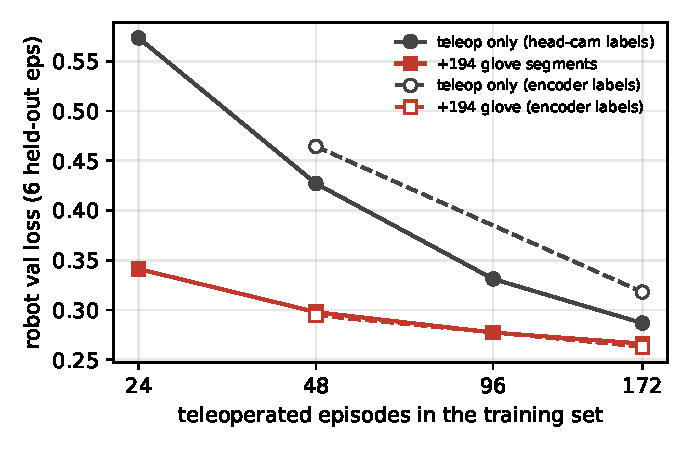
\includegraphics[width=0.6\linewidth]{fig/budget.pdf}
  \caption{Robot validation loss against the number of teleoperated episodes, with and without the 194 glove segments. Solid: head-camera-labelled teleoperation (round-2 chain, four budgets); dashed: encoder-labelled teleoperation (final design, two budgets). The glove set moves every budget to the level of 2--4$\times$ as many teleoperated episodes.}
  \label{fig:budget}
\end{figure}

\begin{figure}[h]
  \centering
  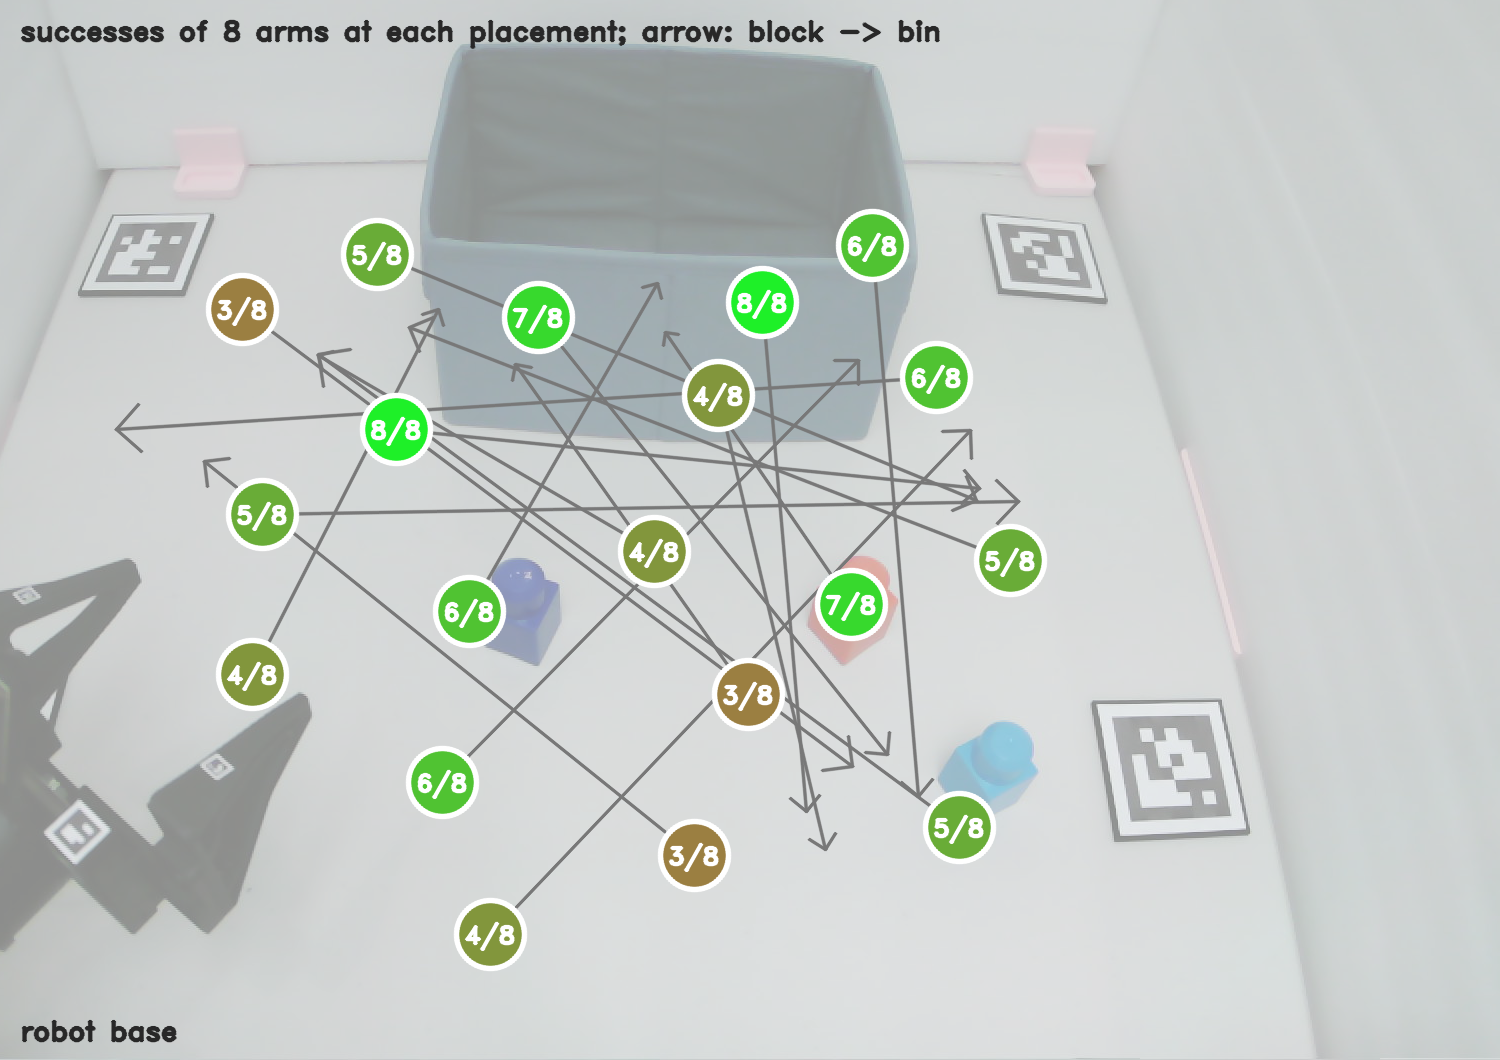
\includegraphics[width=0.58\linewidth]{fig/placements.png}
  \caption{The 25 placements over the fixed camera's view. Each disc is the successes of the eight arms at that placement; the arrow points to the scene's bin.}
  \label{fig:placements}
\end{figure}

\begin{figure}[h]
  \centering
  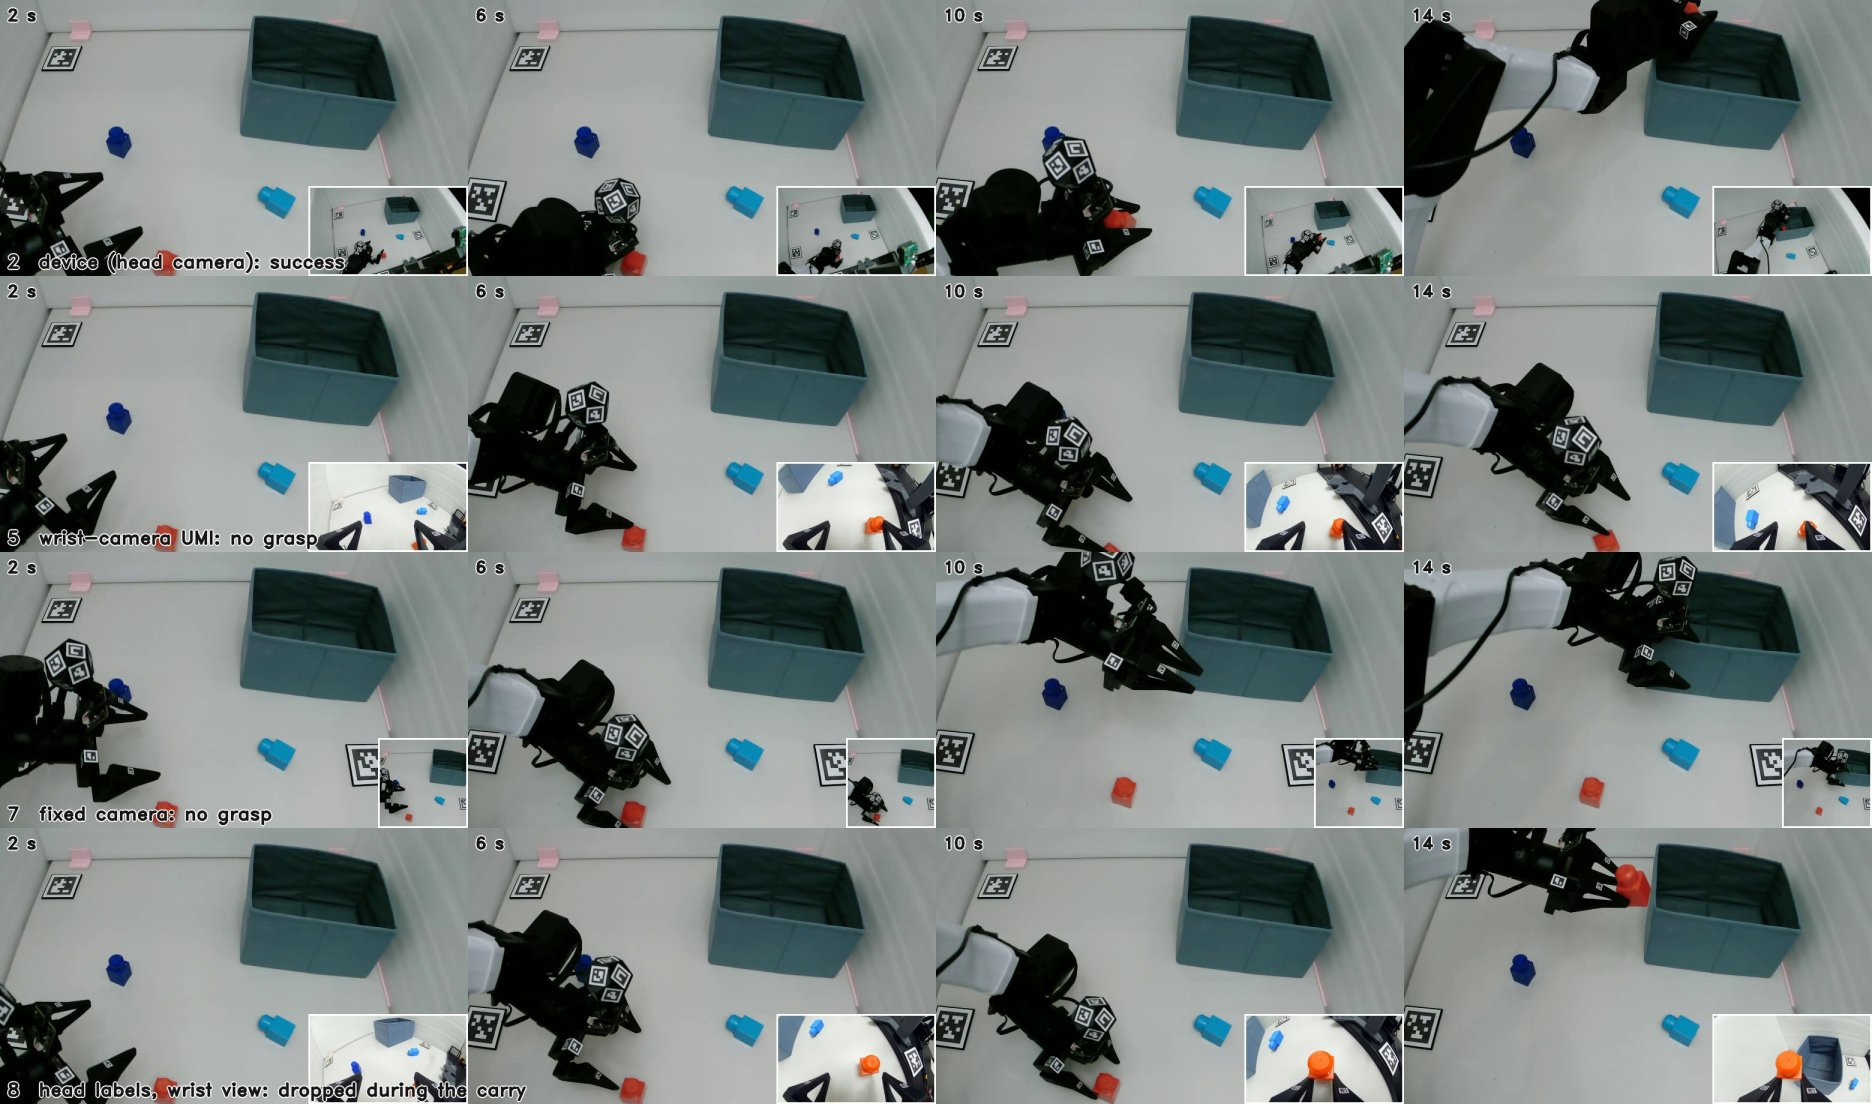
\includegraphics[width=\linewidth]{fig/rollouts.jpg}
  \caption{One placement (scene 16), the four camera arms, at 2, 6, 10 and \SI{14}{s}, from the fixed workspace camera with each policy's own view inset. During the carry the wrist view (rows 2 and 4) holds the block and the far wall and nothing else; the head view (row 1) keeps gripper and bin in one frame. Arm 8 opened with the bin out of its view.}
  \label{fig:rollouts}
\end{figure}
